\chapter{Molecular Dynamics}\label{chap:MD}
Molecular Dynamics (\acrshort{MD}) is an atomistic simulation method that is commonly employed in the investigation of atomic-scale friction due to its ability to track each atom in a system~\cite{Yalin_2011}. In recent years, advances in computing algorithms and hardware have made \acrshort{MD} simulations increasingly capable of simulating tribological systems~\cite{Manini_2016}. We will utilize \acrshort{MD} as our primary numerical approach to examine the frictional behavior of a nanoscale Kirigami sheet sliding on a substrate. The small-scale modifications associated with nanoscale Kirigami are still beyond the reach of experimental approaches, and the complexity of the system precludes analytical solutions as well. Hence, \acrshort{MD} simulations represent one of the few viable options for addressing this problem.

An \acrshort{MD} simulation can be viewed as a ``computational experiment'', where we specify a set of initial conditions and evolve the system to measure certain properties of interest. This is done through the definition of interatomic force fields which allow us to solve Newton's equation
of motion by numerical integration~\cite[p. 303]{BHUSHAN20051507}. Other more sophisticated and accurate approaches exist, like ab initio \acrshort{MD} which utilizes electronic structure calculations at simulation time~\cite{carloni_role_2002}. One of the most popular methods is based on density functional theory (DFT)~\cite{PhysRev.136.B864} which considers quantum mechanical modeling of the electronic state of the system. However, such methods are rarely used in sliding friction simulations since the computational cost makes it only feasible to handle relatively small systems, typically hundreds of atoms, for relatively short durations, typically much less than \SI{1}{ns}~\cite{Vanossi_2013}. In addition, we aim to perform multiple simulations under the
change of various physical parameters which adds extra demands on the computational resources.

In this chapter, we introduce the fundamental principles of \acrshort{MD} modeling and describe our implementation choices for the system of interest. We will focus on the key aspects related to our implementation rather than providing a comprehensive analysis of all available techniques.





% However selecting the appropriate force fields can be a difficult task, since different force fields consider different approximations for the chemical ...


% Ab-initio MD, e.g. of the Car-Parrinello type (Car and Parrinello, 1985), has not really been of use so far in sliding friction, mainly because it can handle only rather small systems, typically hundreds of atoms, for relatively short times, typically ≪ 1 ns. Most MD frictional simulations are therefore based on reasonable empirical interatomic forces (“force fields”), ranging from relatively sophisticated energy surfaces account- ing for electrons at the density-functional level or at the tight-binding level (Xu et al., 1992), to angle-dependent many-particle potentials, to simple pairwise potentials (e.g. Lennard-Jones), to basic simple models of elastic springs, extensions of FK-type formulations.
% https://arxiv.org/abs/1112.3234v4



% A promising compromise could possibly be provided by the so-called reactive
% potentials [120–122], capable of describing some chemical reactions, including
% interface wear with satisfactory computational efficiency in large-scale
% atomic simulations, compared to semi-empirical and first-principles
% approaches. \cite{Manini_2016}



% Despite recent progress in this respect, it is clear that there will always be
% interesting problems beyond the reach of ab initio approaches
% \cite{PhysRevB.37.6991}.


% Physically relevant quantities like the average friction force can be
% evaluated by carrying out averages over the model dynamics. The modeling most
% first of all adress equlibrium and near-equlibrium behvaiour where the
% fluctuation-dissipation theorem governs the conversion of mechanical energy
% into heat. But it most also deal with nonlinear dissipative phenomena such as
% instabilities and stick-slip.\cite{Manini_2016}

% Quantitative data can be obtained by analyzing the numerical output directly.
% [p. 303]{BHUSHAN20051507}





\section{Potentials}\label{sec:potentials}
% \cite{PhysRevB.37.6991}

The interatomic force fields governing the \acrshort{MD} simulation are given from the choice of potentials and have a significant impact on the outcomes obtained. The potentials can vary from intricate energy surfaces that consider electrons at either the density-functional or tight-binding level to angle-dependent many-particle potentials, basic pairwise potentials, or simple models of elastic springs, and extensions of Frenkel-Kontorova-type formulations~\cite{Vanossi_2013}. For the choice of
potentials, and materials, we take a basis in the numerical \acrshort{MD} study
by Li et al.~\cite{li_evolving_2016} simulating a \acrshort{FFM} type setup
where a silicon tip indents a graphene sheet supported by a silicon substrate. Our system obviously differs from this arrangement since we will be sliding the entire sheet upon the substrate. Nevertheless, we contend that this serves as an appropriate basis for selecting the potentials based on the materials involved. Thus, we adopt the potentials from~\cite{li_evolving_2016} describing the covalent bonds between carbon atoms (C--C) in the graphene sheet with the Tersoff potential and the covalent bonds between silicon atoms (Si--Si) in the substrate with the Stillinger–Weber potential. A typical 12--6 Lennard–Jones (\acrshort{LJ}) potential is used to describe the van der Waals adhesive interaction between the graphene sheet and the substrate. 



\subsection{General formulation of potentials}
The potentials determine the interatomic forces in the \acrshort{MD} simulation, with the force $F$ acting on an atom being derived from the potential energy $U$ as the derivative $\vec{F} = -\nabla U$, where $\nabla = (\frac{\partial}{\partial x}, \frac{\partial}{\partial y}, \frac{\partial}{\partial z})$. The energy of $N$ interacting particles can be described as an expansion in terms of participating atoms as 
\begin{align*}
  U = \sum_i V_1(\vec{r}_i) + 
      \sum_{\substack{i, j \\ i < j}} V_2(\vec{r}_i, \vec{r}_j) +  
      \sum_{\substack{i,j,k \\ i < j < k}} V_3(\vec{r}_i, \vec{r}_j, \vec{r}_i) + \cdots,
\end{align*} 
where $\vec{r}_n$ is the position of the $n^{\text{th}}$ particle and $V_m$ is called an $m$-body potential~\cite{PhysRevB.37.6991}. The first one-body term corresponds
to an external potential (e.g.\ gravity), followed by the two-body term, the
three-body term and so on. The simplest model that includes particle interaction
is the pair potential truncating the expansion after the two-body term. A general feature of the pair potentials is that they favor close-packed
structures that are unsuited to describe covalent bonds which take more open
structures. In particular, pair potentials are completely inapplicable to
strongly covalent systems~\cite{PhysRevB.37.6991}. In order to accommodate the
description of covalent bonds we include the three-body term in both the Stillinger–Weber and Tersoff potential. For the interaction between the sheet and the substrate, we use the \acrshort{LJ} pair potential describing the non-bonded van der Waals interaction which is often used to treat interactions between surfaces in friction simulations~\cite{zhu_study_2018,ZHANG201585,Yoon2015MolecularDS,kim_nano-scale_2009}. In the following sections~\crefrange{sec:LJ}{sec:tersoff} we will introduce each of the potentials in more detail.


\subsection{Lennard Jones}\label{sec:LJ}
The theoretical basis in this section is based on~\cite{docs_lammps_LJ,
C9CP05445F, chem_libretexts_LJ}. The Lennard-Jones (\acrshort{LJ}) model is one of the most commonly used pair potentials for \acrshort{MD} simulations. \acrshort{LJ} models the potential energy between two non-bonding atoms solely based on interatomic distance. The model accounts for long-ranged attractive forces arising from London dispersion forces (dipole-induced dipole) and repulsive forces that capture the hard core of overlapping electron orbitals at small distances (Pauli repulsion). Thus, it assumes neutrally charged atoms and was originally proposed for noble gases. The classical 12--6 version of the model, referring to the powers of the repulsive and attractive forces respectively, reads
\begin{align}
  U = 4\epsilon \left[\left(\frac{\sigma}{r}\right)^{12} - \left(\frac{\sigma}{r}\right)^6 \right ], \qquad r < r_c,
  \label{eq:LJ}
\end{align}
where $r$ is the interatomic distance with cut-off $r_c$, $\epsilon$ is the
depth of the potential well and $\sigma$ the interatomic distance where the
the potential is zero. The potential is illustrated in~\cref{fig:LJ_pot}. By solving for the potential minimum ($dU/dr = 0$) we find the equilibrium distance to be $r_0 = \sigma 2^{1/6}$. This makes for a slightly more intuitive interpretation of $\sigma$ as the parameter which sets the equilibrium distance between atoms, i.e.\ the dividing line for which the force is repulsive or attractive. We will adopt the potential parameters from Li et al.~\cite{li_evolving_2016} with $\sigma = \SI{3.0}{\text{Å}}$ and $\epsilon = \SI{0.0092}{eV}$.

\begin{figure}[H]
  \centering
  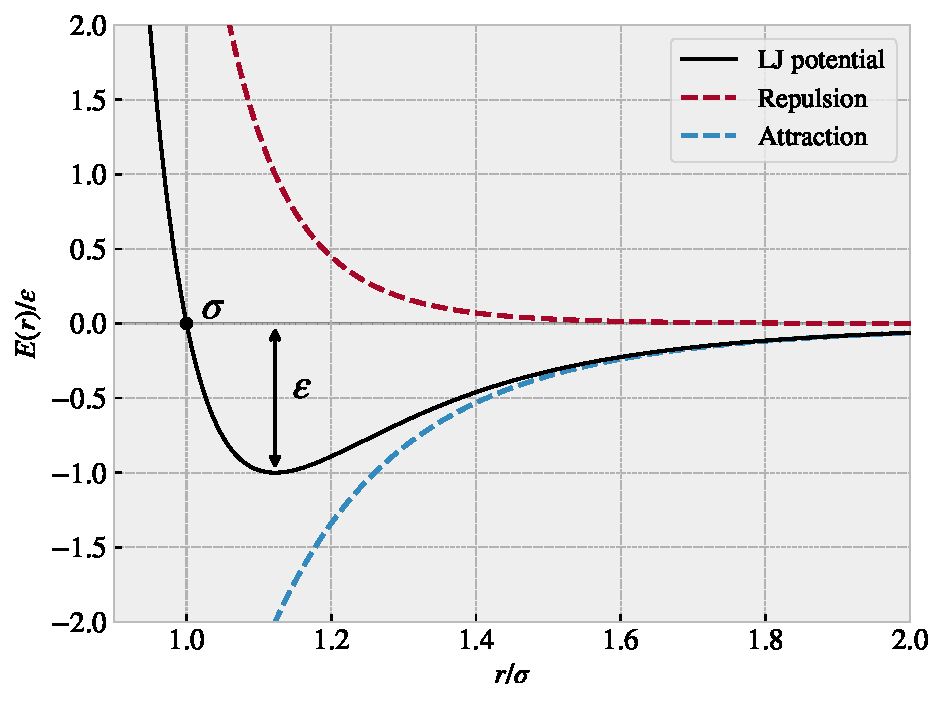
\includegraphics[width=0.6\linewidth]{figures/theory/LJ_pot.pdf}
  \caption{Illustration of the \acrshort{LJ} potential~\cref{eq:LJ} showing the contributions from the repulsive and attractive part of the potential.}
  \label{fig:LJ_pot}
\end{figure}


\subsection{Stillinger-Weber}\label{sec:wb}
The theoretical background of this section is based on~\cite{docs_lammps_sw, PhysRevB.31.5262}. The Stillinger-Weber potential takes the form of a three-body potential
\begin{align*}
  U &=\sum_i \sum_{j>i} \phi_2(r_{i j})+\sum_i \sum_{j \neq i} \sum_{k>j} \phi_3(r_{ij}, r_{ik}, \theta_{ijk}),
\end{align*}
where $r_{ij}$ denotes the distance between atom $i$ and $j$, and $\theta_{ijk}$
the angle between bond $ij$ and $jk$ (see~\cref{fig:three_body_angle}). The summation is over all neighbors $j$
and $k$ of atom $i$ within a cut-off distance $r = a\sigma$. 

\begin{figure}[!htb]
  \centering
  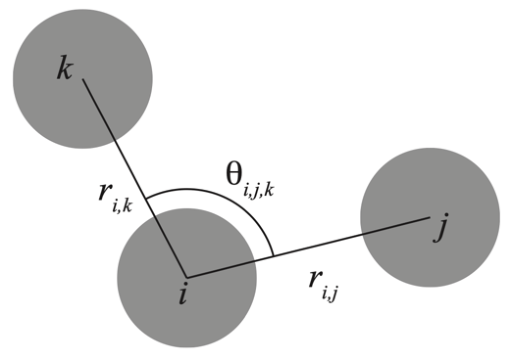
\includegraphics[width=0.35\linewidth]{figures/theory/three_body_angle.pdf}
  \caption{Illustration showing the notation for the distances $r_{ik}$ and $r_{ij}$ and the angle $\theta_{ijk}$ in consideration to the atoms $i$, $j$ and $k$.}
  \label{fig:three_body_angle}
\end{figure}


The two-body term $\phi_2$ builds from the \acrshort{LJ} model with the addition of an exponential cutoff term
\begin{align}
  \phi_2(r_{i j}) & =A_{ij} \epsilon_{ij}\left[B_{ij}\left(\frac{\sigma_{ij}}{r_{ij}}\right)^{p_{ij}} - \left(\frac{\sigma_{ij}}{r_{ij}}\right)^{q_{ij}}\right] \exp (\frac{\sigma_{ij}}{r_{ij}-a_{ij} \sigma_{ij}}).
  \label{eq:sw_2}
\end{align}
The model parameters $A$, $\epsilon$, $B$, $\sigma$, $p$, $q$ and $a$ come with
$i,j$ indices to indicate that these parameters should be specified for each
unique pair of atom types. However, in our case, we will only provide a single
value for each model parameter since we are exclusively dealing with Si--Si bonds. We see that the first term in~\cref{eq:sw_2} is reminiscent of the \acrshort{LJ} model in~\cref{eq:LJ} while the last term effectively drives the potential to zero at $r=a\sigma$, which is the chosen cut-off distance for the potential evaluation. With the chosen model parameters for the Si--Si modeling (see~\cref{tab:sw_param}), the cut-off becomes $\sim \SI{3.8}{\text{Å}}$. The three body term includes an angle dependency as
\begin{align}
  \phi_3(r_{ij}, r_{ik}, \theta_{ijk}) &= \lambda_{ijk} \ \epsilon_{ijk} \Big[\cos \theta_{ijk}-\cos \theta_{0,ijk}\Big]^2 \exp (\frac{\gamma_{ij} \sigma_{ij}}{r_{ij} - a_{ij} \sigma_{ij}}) \exp (\frac{\gamma_{ik} \sigma_{ik}}{r_{ik} - a_{ik} \sigma_{ik}}),
  \label{eq:sw_3}
\end{align}
where $\theta_{0,ijk}$ is the equilibrium angle. The first term of~\cref{eq:sw_3} includes an angle dependency analog to a harmonic oscillator
based on a cosine angle distance from the equilibrium angle. The final two terms
act again as a cut-off function by driving the potential to zero at $r_{ij} =
a_{ij}\sigma_{ij}$ and $r_{ik} = a_{ik}\sigma_{ik}$ respectively. We adopt the parameters for Si--Si modeling suggested in the original paper by Stillinger and Weber~\cite{PhysRevB.31.5262} which is shown in~\cref{tab:sw_param} along with an interpretation of each model parameter.



\begin{table}[H]
  \begin{center}
  \caption{Parameters for the Stilliner-Weber potential used for intermolecular interactions in the silicon substrate. The parameters are adopted from~\cite{PhysRevB.31.5262}.}
  \label{tab:sw_param}
  \begin{tabular}{ | M{2cm} | M{2cm} | X{10cm} |} \hline
    Parameter & Value & Description \\ \hline 
    $\epsilon$ & \SI{2.1683}{eV}  & Depth of the potential well for each pair and triplets of atom types. \\ \hline
    $\sigma$ & \SI{2.0951}{\text{Å}} & Distance for which the individual pair interactions has
    zero potential (analog to the \acrshort{LJ} model). \\ \hline
    $a$ & 1.80 & The cut-off distance for each pair of atom types in units of $\sigma$. \\
    \hline
    $\lambda$ & 21.0 & The overall depth of the three-body potential well. \\
    \hline
    $\gamma$ & 1.20 & The shape of the three-body cut-off terms. \\ \hline
    $\cos{(\theta_0)}$ & -1/3 & Cosine of equilibrium angle. \\ \hline
    $A$ &  7.049556277 & The overall depth of the two-body potential well. \\
    \hline
    $B$ &  0.6022245584 & Scales the repulsion part of the two-body term. \\
    \hline
    $p$  & 4.0 & The power dependency for the repulsion part of the two-body
    term. \\ \hline
    $q$  & 0.0 & The power dependency for the attraction part of the two-body
    term. \\ \hline
    tol  & 0 & (LAMMPS specific) Option to define a different cut-off than the
    theoretical $r = a\sigma$. tol = 0 refers to the use of the theoretical cut-off. \\ \hline
  \end{tabular}
  \end{center}
\end{table}



\subsection{Tersoff}\label{sec:tersoff}
% Add figure similar to:
% https://en.wikipedia.org/wiki/Bond_order_potential#/media/File:Bond-order_interatomic_potential.png,
% showing bond order curves.


% https://interatomic-potentials.readthedocs.io/en/latest/doc/tersoff.html
% https://chem.libretexts.org/Bookshelves/
% Physical_and_Theoretical_Chemistry_Textbook_Maps/Supplemental_Modules_(Physical_and_Theoretical_Chemistry)/Chemical_Bonding/Fundamentals_of_Chemical_Bonding/Bond_Order_and_Lengths


The theoretical basis in this section is based
on~\cite{docs_lammps_tersoff,PhysRevB.37.6991}. The Tersoff potential abandons
the idea of a general $m$-body form and attempts instead to build the model on a
more physics-informed approach; the more neighbors an atom has the weaker the
bonds will be. Thus, it introduces the bond order (bond strength), which is
environment specific and decreases with increasing bond coordination (number of
neighbors for a given atom). A sketch of the Tersoff potential can be seen
in~\cref{fig:bond_order}. 


\begin{figure}[!htb]
  \centering
  \includegraphics[width=0.6\linewidth]{figures/theory/Bond-order_interatomic_potential.png}
  \caption{Sketch of the potential energy for a Tersoff-type potential. The energy minimum is shifted with changing bond order $b_{ijk}$. Reproduced from~\cite{wiki:bond_order}.}
  \label{fig:bond_order}
\end{figure}


The potential energy is taken to have the form
\begin{align*}
  U &= \sum_i U_i = \frac{1}{2}\sum_{i \ne j} V_{ij}, \\
  V_{ij} &= f_C(r_{ij}) \big[f_R(r_{ij}) + b_{ij}f_A(r_{ij})  \big],
\end{align*}
where the total potential energy $U$ is decomposed into a bond energy $V_{ij}$.
The indices $i$ and $j$ run over the atoms of the system with $r_{ij}$ denoting
the distance between atom $i$ and $j$. Notice that the sum includes all
combinations of $i,j$ but $i\ne j$, meaning that an atom cannot bond to itself.
However, we count other bonds twice, e.g.\ $(1,2)$ and $(2,1)$, which is the
explanation for the additional factor $1/2$. The reasoning for the double
counting lies in the asymmetry of the bond order $b_{ij}\ne b_{ji}$ leading to
$V_{ij}\ne V_{ji}$. The bond energy is composed of a repulsive term $f_R$,
arising from overlapping wave functions, and an attractive term $f_A$ associated
with bonding. $f_C$ is simply a smooth cut-off function to increase
computational efficiency. $b_{ij}$ represent the bond order, i.e.\ the strength
of the bonds, which depends inversely on the number of bonds, the bond angles
($\theta_{ijk}$) and optionally the relative bond lengths ($r_{ij}$, $r_{jk}$).
Notice that an additional cut-off term $a_{ij}$ was originally multiplied to
$f_R$ as a way of limiting the range of the repulsive interactions to
the first neighbor shell. This is similar to the role of $b_{ij}$ for the attractive term $f_A$, but it is often omitted for the repulsive
term $f_R$, and we do so as well by setting $a_{ij} = 1$. 

The cut-off function $f_C$ goes from 1 to 0 over a small interval range $R \pm
D$ as
\begin{align*}
  f_C(r) =
  \begin{cases}
    1 & r < R - D \\
    \frac{1}{2} - \frac{1}{2} \sin{(\frac{\pi}{2} \frac{r - R}{D})} & R - D < r < R + D\\
    0 & r > R + D
  \end{cases},
\end{align*}
which is continuous and differentiable for all $r$. $R$ is usually chosen to
include only the first neighbor shell. \\
The repulsive and attractive terms $f_R$ and $f_A$ are modeled as an exponential
function, similar to a Morse potential, 
\begin{align*}
 f_R(r) &= A \exp(-\lambda_1 r), \\
 f_A(r) &= -B \exp \big(-\lambda_2 r\big).
\end{align*}
The novel feature of the Tersoff model lies in the modeling of the bond order
$b_{ij}$ which includes three-body interactions by summing over a third atom $k
\ne i,j$ within the cut-off $r_{ik} < R + D$ as shown in the following.
\begin{align}
  b_{i j} & =\big(1+\beta^n \zeta_{i j}^n\big)^{-\frac{1}{2 n}} \\
  \zeta_{i j} & =\sum_{k \ne i,j} f_C(r_{i k}) g\Big(\theta_{i j k}\left(r_{i j}, r_{i k}\right)\Big) \exp \left(\lambda_3{ }^m\big(r_{i j}-r_{i k}\right)^m\big) \\
  g(\theta) & =\gamma_{i j k}\left(1+\frac{c^2}{d^2}-\frac{c^2}{\left[d^2+\left(\cos \theta-\cos \theta_0\right)^2\right]}\right).
  \label{eq:tersoff_bond_order}
\end{align}
In~\cref{eq:tersoff_bond_order} $\zeta_{i,j}$ is an effective coordination and
$g(\theta)$ captures angle dependency and is minimized at the equilibrium
angle $\theta = \theta_0$. The parameters used to model the graphene C--C bonds
are adopted from J.\ Tersoff~\cite{PhysRevB.39.5566} and summarized in
\cref{tab:tersoff_param}.

\begin{table}[H]
  \begin{center}
  \caption{Parameters for the Tersoff potential used for intermolecular interactions in the graphene sheet. The parameters are adopted from~\cite{PhysRevB.39.5566}.}
  \label{tab:tersoff_param}
  \begin{tabular}{ | M{2cm} | M{2cm} | X{9cm} |} \hline
    Parameter & Value & Description \\ \hline 
    $R$ & 1.95 Å & Center distance for cut-off. \\ \hline
    $D$  & 0.15 Å & Thickness of cut-off region. \\ \hline
    $\lambda_1$ & 3.4879 Å$^{-1}$ & Decay of repulsion potential term $f_R$. \\ \hline
    $\lambda_2$ & 2.2119 Å$^{-1}$ & Decay of attractive potential term $f_A$. \\ \hline
    $A$ & 1393.6 eV & Repulsion potential maximum at the core ($f_R(r_{ij} = 0)$). \\ \hline
    $B$ & 346.74 eV & Attractive potential minimum at core ($f_A(r_{ij} = 0)$). \\ \hline
    $\beta$ & \num{1.5724e-7} & Base for the exponential scaling of the effective coordination effect on bond strength $b_{ij}$. \\ \hline
    $n$ & 0.72751 & Power law exponent for the bond order dependency. \\ \hline
    $\lambda_3$ & 0.0 Å$^{-1}$ & Base for the exponential cut-off of the effective coordination $\zeta_{ij}$. \\ \hline
    $m$ & --- & Exponent for the exponential cut-off of the effective coordination $\zeta_{ij}$. Not relevant since $\lambda_3 = 0$. \\ \hline
    $\gamma$ & 1.0 & Linear scaling of the angle dependecny term. \\ \hline
    $c$ & \num{3.8049e4} & Strength of the angular effect. \\ \hline
    $d$ & 4.3484 & Determines the ``sharpness'' of the angular dependency. \\
    \hline
    $\cos{(\theta_0)}$ & $-0.57058$ & Cosine of the equilibrium angle. \\ \hline
  \end{tabular}
  \end{center}
\end{table}





\section{Integration}\label{sec:integration}
Assuming that one has defined a system of atoms, defining the atom types, initial positions and velocities, and interatomic potentials, we need
to move the system forward in time. By solving Newton's equations of motion we achieve this by effectively sampling the microcanonical ensemble characterized by a constant number of particles $N$, volume $V$ and energy $E$, hence denoted $NVE$~\cite{dfrenkel96:mc}. Newton's equations of motion read
\begin{align}
  m_i \frac{d^2 \vec{r}_i}{dt^2} = \vec{F}_i = -\nabla U_i,
  \label{eq:NE}
\end{align}
where $i$ is the atom index, $m_i$ its mass, $\vec{r}_i = (x_i, y_i,
z_i)$ the position, $t$ is time, $\nabla_i = (\frac{\partial}{\partial x_i},
\frac{\partial}{\partial y_i}, \frac{\partial}{\partial z_i})$ and $U_i$ the
potential energy. The potential energy is defined by the interatomic potentials and any external forces applied to the system. Since the forces defined by the potentials are conservative we expect the energy of the solution
to be conserved. We can redefine~\cref{eq:NE} in terms of two coupled first
order differential equations 
\begin{align}
  \dot{\vec{v}}_i(t) = \frac{\vec{F}}{m_i}, \qquad \dot{\vec{r}}_i(t) = \vec{v}_i(t),
  \label{eq:NE_2}
\end{align}
where $\dot{x} = dx/dt$ is Newton's notation for the time derivative and $\vec{v} = (v_x,v_y,v_z)$ is velocity. Numerically we can solve the coupled equations by integrating over discrete timesteps. That is, we discretize the solution into temporal steps $t_k = t_0 + k\Delta t$ with start time $t_0$ and timestep $\Delta t$. The choice of timestep should be chosen small enough to avoid instabilities in the numerical solution.


\subsection{Velocity Verlet}
% http://www.physics.drexel.edu/~valliere/PHYS305/Diff_Eq_Integrators/Verlet_Methods/Diffrntleqn3.pdf
% https://www2.ph.ed.ac.uk/~dmarendu/MVP/MVP03.pdf

A popular approach to the numerical integration of Newton's equations of motion, when written as two coupled first-order differential equations~\cref{eq:NE_2}, is the \textit{velocity verlet} algorithm. We can derive the algorithm by the use of Taylor expansions. We begin by expanding the next-step position vector $\vec{r}_i(t + \Delta t)$ at time $t$
\begin{align}
  \vec{r}_i(t + \Delta t) &= \vec{r}_i(t) + \dot{\vec{r}}_i(t) \Delta t + \frac{\ddot{\vec{r}}_i(t)}{2} \Delta t^2 + \mathcal{O}(\Delta t^3) \label{eq:vv_comp1},
\end{align}
where $\ddot{\vec{r}} = d^2\vec{r}/dt^2$ and $\Delta t^n$ is simply the relaxed
notation for $(\Delta t)^n$. The remaining $\mathcal{O}(\Delta t^3)$ term is big O notation for the truncation including a dependence of $\Delta t^3$ and higher order. Similarly, we take the expansions of the next-step
velocity vector $\vec{v}_i(t+\Delta t)$ at time $t$ 
\begin{align}
  \vec{v}_i(t+\Delta t) = \vec{v}_i(t) + \dot{\vec{v}}_i(t) \Delta t + \frac{\ddot{\vec{v}}_i(t)}{2}\Delta t^2 + \mathcal{O}(\Delta t^3).
  \label{eq:tay_v1}
\end{align}
Finally, by taking the expansion of $\dot{\vec{v}}_i(t+\Delta t)$ we can
eliminate the $\ddot{\vec{v}}_i$-term in~\cref{eq:tay_v1} and simplify it as
shown in the following.
\begin{align}
  \dot{\vec{v}}_i(t+\Delta t) &= \dot{\vec{v}}_i(t) + \ddot{\vec{v}}_i(t) \Delta t + \mathcal{O}(\Delta t^2) \nonumber \\
  \frac{\ddot{\vec{v}}_i(t)}{2}\Delta t^2 &= \frac{\Delta t}{2}\Big( \dot{\vec{v}}(t+\Delta t) - \dot{\vec{v}}_i(t)\Big) + \mathcal{O}(\Delta t^3) \nonumber \\
  &\Downarrow \nonumber \\
  \vec{v}_i(t+\Delta t) &= \vec{v}_i(t) + \dot{\vec{v}}_i(t) \Delta t + \frac{\Delta t}{2}\Big( \dot{\vec{v}}_i(t+\Delta t) - \dot{\vec{v}}_i(t)\Big) + \mathcal{O}(\Delta t^3) \nonumber \\
  &=  \vec{v}_i(t) + \frac{\Delta t}{2}\Big( \dot{\vec{v}}_i(t) +  \dot{\vec{v}}_i(t+\Delta t)\Big) + \mathcal{O}(\Delta t^3).
  \label{eq:vv_comp2}
\end{align}
By combining~\cref{eq:vv_comp1} and~\cref{eq:vv_comp2} using $\dot{\vec{v}} = \vec{F}_i(t)/m_i$ and $\vec{v} = \dot{\vec{r}}$ we
arrive at the final scheme
\begin{align*}
  \vec{r}_i(t + \Delta t) &= \vec{r}_i(t) + \vec{v}_i(t) \Delta t + \frac{\vec{F}_i(t)}{2m_i}\Delta t^2 + \mathcal{O}(\Delta t^3), \\
  \vec{v}_i(t+\Delta t)  &= \vec{v}_i(t) + \frac{\vec{F}_i(t) + \vec{F}_i(t+\Delta t)}{2m_i}  \Delta t + \mathcal{O}(\Delta t^3).
\end{align*}
This scheme will give a local error on the order $\Delta t^3$ corresponding to a
global error of $\Delta t^2$. One of the most popular ways to implement this
numerically is as stated in the following steps.
\begin{enumerate}[leftmargin=6cm]
  \item Calculate $v_{k+\frac{1}{2}} = v_k + \frac{F_k}{2m} \Delta t$.
  \item Calculate $r_{k+1} = r_k + v_{k+\frac{1}{2}} \Delta t$.
  \item Evaluate the force $F_{k+1} = F(r_{k+1})$.
  \item Calculate $v_{k+1} = v_{k+\frac{1}{2}} + \frac{F_{k+1}}{2m} \Delta t$  
\end{enumerate}



\section{Thermostats}\label{sec:thermostat}
In~\cref{chap:friction} we introduced friction as an ultimate result of the equipartition theorem stating that the kinetic energy supplied by the sliding motion will tend to transfer to other degrees of freedom and eventually dissipate to the environment as heat through phonon transport (and electrons for a metallic system)~\cite{Manini_2016}. However, when modeling the system exclusively through the solutions of Newton's equations of motion we have no dissipation channel in our system. Instead, the energy will reflect back and forth and eventually ``pile up'' in the system in an unphysical manner. In order to resolve this issue we have to model the heat dissipation to the environment. This can be approached in a variety of ways, but one of the more common choices, which we will use as well, is the Langevin thermostat.


% Thus, we need to add an energy sink representing the bulk material sourronding the system of interest, which let the heat dissipate add a steady state. 


% In order to model a realistic friction response we must ensure that excitations in the system is allowed to
% propagate in the system and disperse in the bulk of both sheet and substrate.
% Due to a relatively small simulation size theese are likely to relflect back and ``pile up'' unphysically.

% Thus in order to avoid continuous heating and attain a steady state
% the (Joule) heat must be removed at a steady state. This is very the viscous
% damping of the langevin equations enter the picture. It can be difficulut to set
% the value $\gamma$ for the magnitude of this damping. The unphysical
% introduction of heat sink can be mittigated by some modifictions he mention,
% which is kind of next level I guess. 


\subsection{Langevin thermostat} \label{sec:langevin}

% Check out \cite{Manini_2016} for a good theory section on this that I had
% completely missed when writing this!

% Based on
% https://www.uio.no/studier/emner/matnat/fys/FYS4130/v19/pensumliste/stat-phys_2019.pdf

% http://physics.gu.se/~frtbm/joomla/media/mydocs/LennartSjogren/kap6.pdf

The Langevin thermostat is a stochastic thermostat that modifies Newton's
equation of motion such that the solution lies in the canonical ensemble
characterized by a constant number of particles $N$, constant volume $V$ and
constant temperature $T$, hence denoted $NVT$~\cite{Manini_2016}. When going from the microcanonical ensemble $NVE$, described by Newton's equation of motion~\cref{eq:NE}, to the canonical ensemble $NVT$, we effectively perform a Legendre transformation which substitutes temperature for energy in the regard to which variables are held constant. The canonical ensemble is represented by a finite system being in contact with an infinite heat bath of temperature $T$. The $NVT$ ensemble is equivalent to sampling a system in thermodynamic equilibrium where the weight of each microscopic state is given by the Boltzmann factor $\exp[-E/(k_B T)]$ where $k_B$ is the Boltzmann constant. 

The Langevin thermostat is governed by the Langevin equation which originated as the modified version of Newton's equations for a Brownian particle~\cite{stat_phys}. A Brownian particle is a small particle suspended in liquid,
e.g.\ pollen or dust, named after Robert Brown (1773–1858) who was the first to
observe its jittery motion. The Langevin equation describes this motion as the
combination of a viscous drag force $ -\alpha \vec{v}$, where $\alpha$ is a
positive friction coefficient and $\vec{v}$ the velocity vector, and a random
fluctuation force $\vec{R}$. The Langevin equation reads
\begin{align}
  m \frac{d \vec{v}}{dt} = -\alpha \vec{v} + \vec{R},
  \label{eq:Langevin}
\end{align}
where $m$ is the particle mass. This effectively describes the particle of
interest, the Brownian particle, as being suspended in a sea of smaller
particles. The collision with these smaller particles is modeled by the combined effects of the drag force and the fluctuation force. If the fluctuation force is excluded~\cref{eq:Langevin} becomes 
\begin{align*}
  m \frac{d \vec{v}}{dt} = -\alpha \vec{v} \quad \Rightarrow \quad 
  \vec{v}_i(t) = v(0)e^{- \frac{\alpha t}{m}},
\end{align*}
where the solution reveals that the Brownian particle will come to a complete stop
after a long time ${\vec{v}_i(t\to\infty) \to \vec{0}}$. This is in violation
with the equipartition theorem which dictates a non-zero average squared velocity in equilibrium $\langle v^2 \rangle_{\text{eq}}$ as
\begin{align}
  \frac{1}{2}m\langle v^2 \rangle_{\text{eq}} = \frac{k_B T}{2}.
  \label{eq:equipartion}
\end{align}
Hence, the fluctuation force is necessary to obtain the correct equilibrium. In the following, we will attempt to introduce the reasoning behind the Langevin equations using only one dimension in order to simplify the notation a bit. This is based on~\cite{stat_phys}.

We describe the statistical nature of the collisions as a sum of
independent momentum transfers
\begin{align*}
  \Delta P = \sum_i^N \delta p_i,
\end{align*}
where $\Delta P$ denotes the change of momentum after $N$ momentum transfers
$\delta p_i$ from the environment to the Brownian particle. We assume the first
and second moments to be $\langle \delta p \rangle = 0$ and  $\langle \delta p \rangle
= \sigma^2$. When $N$ is large the central limit theorem states that the random
variable $\Delta P$ has a gaussian distribution with  $\langle P \rangle = 0$
and $\langle \Delta P^2 \rangle = N\sigma^2$. If we consider the momentum change
$\Delta P$ over a discrete time $\Delta t$, where the number of collisions is
proportional to time $N \propto \Delta t$, the corresponding fluctuation force
$R = \Delta P / \Delta t$ will have a variance 
\begin{align*}
  \langle R^2 \rangle = \frac{\langle \Delta P^2 \rangle}{\Delta t^2} = \frac{N \sigma^2}{\Delta t^2}  \propto \frac{1}{\Delta t}.
\end{align*}
In an \acrshort{MD} simulation, we pick a random force $R(t)$ from a Gaussian
distribution every timestep $\Delta t$. These forces will not be correlated as
long as $\Delta t$ is larger than the correlation time of the forces from the molecular fluid. By assuming that this criterion is met we can write the correlation function as 
\begin{align}
  \langle R(t) R(0) \rangle = 
  \begin{cases}
    \frac{a}{\Delta t}, & |t| < \Delta t/2 \\
    0, & |t| > \Delta t/2,
    \label{eq:disc_corr}
  \end{cases}
\end{align}
where the constant $a$ describes the magnitude of the fluctuations. We could in principle determine $a$ from the variance of $\Delta P$, but instead, we will determine it from the equipartition principle. In the limit $\Delta t \to 0$ the correlation function becomes
\begin{align}
  \langle R(t)R(0) \rangle = a \delta(t),
  \label{eq:F_corr}
\end{align}
% Note that the delta function is justified by the fact that the characteristic
% frequencies of the phonon and electron excitations are much shorter than the
% hopping rate of the tip between the minima of the interaction potential
% \cite{gnecco_meyer_2015}
where $\delta$ denotes the Dirac delta function. This is valid for all spatial
coordinates which are all independent of each other. Since both the drag
force and the fluctuation force originate from the molecular fluid, where the
drag force $-\alpha \vec{v}$ carries a velocity dependency, it is reasonable to assume that fluctuation force is independent of velocity, i.e. $\langle R_i v_j \rangle = 0$ for all cartesian indices $i$ and $j$. In the following, we attempt to justify the physical motivation for the Langevin equation by determining the relationship between the drag coefficient $\alpha$ and the random force $R$~\cite{stat_phys}. From the Langevin equation~\cref{eq:Langevin} we can compute the velocity autocorrelation function. Note that we continue to use only one dimension for simplicity. We begin by multiplying by $(e^{\alpha t /m})/m$
\begin{align*}
  \dot{ v}(t)e^{\alpha t /m} + \frac{\alpha}{m} v(t)e^{\frac{\alpha t}{m}}  = \frac{ F}{m}e^{\frac{\alpha t}{m}}.
\end{align*}
We integrate from $t = -\infty$, using integration by parts on the
latter term on the left-hand side, in order to calculate the velocity 
\begin{align*}
  \int_{-\infty}^t dt' \ \dot{ v}(t')e^{\frac{\alpha t'}{m}} + \frac{\alpha}{m} v(t)e^{\frac{\alpha t'}{m}} &=  \int_{-\infty}^t dt' \ e^{\frac{\alpha t'}{m}} \frac{ F(t')}{m}  \\
  \int_{-\infty}^t dt' \ \dot{ v}(t')e^{\frac{\alpha t'}{m}} + \left(\Big[ v(t')e^{\frac{\alpha t'}{m}}\Big]_{-\infty}^t - \int_{-\infty}^t dt' \ \dot{ v}(t')e^{\frac{\alpha t'}{m}}\right) &= \int_{-\infty}^t dt' \ e^{\frac{\alpha t'}{m}} \frac{ F(t')}{m}  \\
   v(t) &= \int_{-\infty}^t dt' \ e^{\frac{-\alpha(t - t')}{m}} \frac{ F(t')}{m},
\end{align*}
where $e^{\frac{-\alpha t}{m}}$ plays the role of a response function. We can
then calculate the autocorrelation 
\begin{align*}
  \big\langle  v(t) v(0) \big\rangle &= \int_{-\infty}^t dt_1 \ \int_{-\infty}^0 dt_2 \ e^{\frac{t - t_1 - t_2}{m}} \frac{\langle  F(t_1)  F(t_2) \rangle}{m^2} \\
  &= \int_{-\infty}^t dt_1 \ \int_{-\infty}^0 dt_2 \ e^{\frac{t - t_1 - t_2}{m}} \frac{a \delta(t_1 - t_2)}{m^2} \\
  &= \int_{-\infty}^0 dt_2 \ e^{\frac{t - 2t_2}{m}} \frac{a}{m^2} = \frac{a}{2m\alpha}e^{-\frac{\alpha t}{m}},
\end{align*}
where we used~\cref{eq:F_corr} and the fact that the integration commutes with
the average (we are allowed to flip the order). By comparing this with the
equipartition theorem we get 
\begin{align*}
  \frac{1}{2}m\langle  v^2 \rangle &= \frac{k_BT}{2} \\
  \frac{1}{2}m\langle  v(0) v(0) \rangle = \frac{a}{4\alpha} &= \frac{k_BT}{2} \\
  a &=  2\alpha k_B T 
\end{align*}
We notice the appearance of $\alpha$ meaning that the magnitude of the
fluctuations increase both with viscous friction ($-\alpha \vec{v}$) and temperature $T$. Moreover, we can
integrate the velocity over time to get displacement $x(t)$ and show that the
variance is~\cite{stat_phys}
\begin{align*}
  \big\langle x^2(t) \big\rangle = \frac{2 k_B T}{\alpha} \left(t - \frac{m}{\alpha}\left(1 - e^{-\alpha t/m} \right) \right).
\end{align*}
For $t \gg m/\alpha$, only the $t$-term will survive yielding
\begin{align*}
  \langle x^2(t) \rangle = 2 k_BTt/\alpha.
\end{align*}
In 1D, the diffusion constant $D$ is related to the variance as $\langle x^2
\rangle = 2Dt$, meaning that this represents the Einstein relation $D = \mu k_B
T$ with the mobility $\mu = 1/\alpha$. When $t \ll m/\alpha$, we use the Taylor expansion $1 - e^{-x} \approx x - x^2/2$
for $x\ll 1$ which gives
\begin{align*}
  \big\langle x^2(t) \big\rangle = \frac{k_B T}{m} t^2.
\end{align*}
Using $\langle x^2 \rangle / t^2 = \langle v^2 \rangle$ we see that the result is in agreement with the equipartition theorem~\cref{eq:equipartion}
\begin{align*}
  \big\langle v^2(t) \big\rangle = \frac{k_B T}{m} \ \Longleftrightarrow \ \frac{1}{2}m\langle v^2 \rangle_{\text{eq}} = \frac{k_B T}{2}.
\end{align*}
Thus, we find the finite correlation time $\alpha/m$ to describe the crossover from the ballistic regime $\sqrt{\langle x^2(t)
\rangle} \propto \sqrt{t}$ at $t \ll m/\alpha$ to the diffusive regime $\sqrt{\langle x^2(t)\rangle} \propto \sqrt{t}$ at $t \gg m/\alpha$. That is, at short time scales the thermal movement can be thought of as relatively free with a low collision rate, while at longer time scales the movement is characterized by a jittery random-walk-looking motion that is related to diffusion. 


% What do we use for this in the simulation?


% Introduce the fluctuation-dissipation theorem concept earlier since this is a
% motivaiton for the Langeivn equation. 


% Of course, this approach is not rigorous, since the relevant particles
% colliding with each given simulated atom are already all included in the
% conservative and deterministic forces explicitly accounted for by the “force
% field”. The Langevin approach is quite accurate to describe small
% perturbations away from equilibrium, but it may fail quite badly in the
% strongly out-of-equilibrium nonlinear phenomena which are the target of the
% present paper.  \cite{Manini_2016}

\subsection{Implementing Langevin}
% https://docs.lammps.org/fix_langevin.html

% https://www2.ph.ed.ac.uk/~dmarendu/MVP/MVP03.pdf

% https://chem.libretexts.org/Bookshelves/Physical_and_Theoretical_Chemistry_Textbook_Maps/Non-Equilibrium_Statistical_Mechanics_(Cao)/01%3A_Stochastic_Processes_and_Brownian_Motion/1.04%3A_The_Langevin_Equation

% \cite{Hunenberger2005}(pp. 115, 120-121) \cite{docs_lammps_langevin}

The numerical implementation of the Langevin equation~\cref{eq:Langevin} is done through the simulation software LAMMPS (see~\cref{sec:LAMMPS}) following~\cite{PhysRevB.17.1302} by defining the force vector for each particle as 
\begin{align}
  \vec{F} &= \vec{F_c} + \vec{F}_{f} + \vec{F}_{r} \nonumber \\
  &= -\nabla U - \gamma m \vec{v} + \sqrt{\frac{2 k_B T m \gamma}{\Delta t}}\vec{h}(t)
  \label{eq:Langevin_generalized}
\end{align}
where $\vec{F_c}$ is the added conservative force computed via the usual
interatomic interactions described by the potential $U$, $\vec{F}_f$ is the
drag force described as a damping term $-\gamma m \vec{v}$ with $\alpha = \gamma m$, and $\vec{F}_r$ is the random fluctuation force where $\vec{h}$ is a random vector drawn from a normal distribution with zero mean and unit variance. The fact that $\Delta t$ now appears in the denominator for the random force variance $2k_B T m \gamma / \Delta t$ is due to the discretization of time. By applying~\cref{eq:Langevin_generalized} we get the refined velocity verlet scheme
\begin{align*}
  \vec{v}_i(t + \Delta t/2)  &= \vec{v}_i(t) - \frac{\Delta t}{2}\left(\frac{\nabla_i U(t)}{m_i} + \gamma \vec{v}_i \right) + \sqrt{\frac{k_B T \gamma \Delta t}{2m_i}} \vec{h}_i \\ 
  \vec{r}_i(t + \Delta t) &= \vec{r}_i(t) + \vec{v}_i(t + \Delta t/2) \Delta t \\
  \vec{v}_i(t + \Delta t) &= \vec{v}_i(t+ \Delta t/2) - \frac{\Delta t}{2}\left(\frac{\nabla_i U(t + \Delta t)}{m_i} + \gamma \vec{v}_i(t + \Delta t/2) \right) + \sqrt{\frac{k_B T \gamma \Delta t}{2m_i}} \vec{h}_i
\end{align*}
% A little unsure whether the factor 2 in the denominator in the random force is
% correct.
with new random vector $\vec{h}_i$ for each particle and each update. Notice
however, we will only apply the thermostat to specific regions in our simulation, mainly on the outer edges, while the main part of interest is modeled exclusively by Newton's equation of motion as described in~\cref{eq:NE}. This is done in order to avoid affecting the governing parts of the friction simulation too much. We use a damping of $1/\gamma = m/\alpha = \SI{1}{ps}$ as a common default choice. 


% In practice the implementation of the thermostat is implemented discretely by
% updating the force on each particle by the addition of the described forces
% $f_f$ and $f_r$ for each particle. In LAMMPS this is controlled by the user
% defined damping factor ``damp'' = $\gamma^{-1}$ in units of time whih control
% how fast we are going to reach the temperature equlibrium. Thus the
% documentation (\cite{docs_lammps_langevin}) defines the added forces as


% https://www2.ph.ed.ac.uk/~dmarendu/MVP/MVP03.pdf
% https://www.uio.no/studier/emner/matnat/fys/FYS4130/v19/pensumliste/stat-phys_2019.pdf

% ``The Langevin equation is Newtons second law for a Brownian particle, where
% the forces include both the viscous drag due to the surrounding fluid and the
% fluctuations caused by the individual collisions with the fluid molecules.''

% % http://physics.gu.se/~frtbm/joomla/media/mydocs/LennartSjogren/kap6.pdf
% % https://www2.ph.ed.ac.uk/~dmarendu/MVP/MVP03.pdf ``Another option to
% simulate a system in the NVT ensemble is to use a stochastic thermostat, as
% opposed to the deterministic thermostat defined through the Nose-Hoover
% equations.''

% see https://www2.ph.ed.ac.uk/~dmarendu/MVP/MVP03.pdf p. 4


\section{Limitations}
On a general note, \acrshort{MD} simulations are limited to relatively small
time and size scales due to the available computation time. Morden CPUs perform
on the order of \num{e9} floating-point operations per second (FLOPS) per core~\cite{Vanossi_2013}. \acrshort{MD} simulations can benefit from medium-scale
parallelization, demonstrating relatively linear scaling up to around $10^2$
cores, providing roughly $10^{11}$ FLOPS. In a typical \acrshort{MD} calculation, the computation of the force acting on each atom, which can be the most time-consuming step depending on the complexity and range of the force field, requires $N_{\text{step}}$ steps being approximately 10 to $10^2$ FLOPS. Therefore, for a typical simulation size of $N = \num{e5}$ atoms with a timestep in the fs range, we find the ratio of simulated time to real-time on the order 
\begin{align*}
  \frac{\text{FLOPS}}{N\cdot N_{\text{step}} \cdot dt^{-1}} \sim \frac{\num{e11}}{\num{e5}\cdot 10 \cdot \num{e15}} = \num{e-10}.
\end{align*}
Hence, the simulation can make progress at a rate of \SI{100}{ps} per second, or roughly $\SI{e9}{fs}=\SI{1}{\mu s}$ per day. This serves as a rough estimate for the capabilities of \acrshort{MD} simulations. Regarding the ``realism'' of the simulations, some general weaknesses include the lack of considering quantum effects and a reduction in the number of dissipation channels available.


% \cite{Yalin_2011}. Thus, the weaknesses
% include the lack of quantum effects.

% Weak- nesses include a lack of quantum effects in classical atomistic
% dynamics, and perhaps more importantly, the fact that meaningless results can
% be obtained if the simulation conditions are incorrectly chosen. \cite[p.
% 303]{BHUSHAN20051507}



% Read Size- and time-scale issues
% https://arxiv.org/abs/1112.3234v4


% Speed
% Dissipation

% Adding viscous friction in the modelling of friction seems like an obvious issue for a true picture of this. The simplicity of the dissipation channel might be of importance for the final results. 

% One of the limitations of concern is in regard to the simulation scale.
% Despite relatively fast processor speed and efficient algorithm the number of
% atoms that can be handled realistically is still insufficient for complex
% system simulation \cite{kim_nano-scale_2009}.



% The main problem when studying the velocity dependence of friction by MD
% simulations is the fact that speeds below few m/s are not accessible. These
% values are well above typical speeds at which atomic stick–slip is resolved by
% AFM (nm/s to μm/s). The reason for that is the typical time scales in MD,
% which are of the order of 1 fs. Furthermore, phenomena such as thermally
% activated hopping are not effective at high speeds, which makes any attempts
% to extrapolate the model predictions on the velocity dependence of friction
% quite doubtful. A possible solu- tion consists of accelerating the simulations
% during the long stick phases separating rapid slip events. \cite[p.
% 207]{gnecco_meyer_2015}


\section{LAMMPS}\label{sec:LAMMPS}
For the implementation of our \acrshort{MD} we use LAMMPS (Large-scale Atomic/Molecular Massively Parallel Simulator)~\cite{LAMMPS}. LAMMPS provides a numerical framework for setting up the system and integrating the equations of motion with easy access to parallelization of the simulations. This essentially allows us to focus on the higher-level features of the numerical procedure rather than writing the code from scratch. 